\section*{Methods}
%%% https://www.nature.com/sdata/submission-guidelines
% - steps or procedures used to create the data, including full descriptions of the experimental design, data acquisition and any computational processing. 
% - For secondary datasets compiled from other sources, all details of input data should be described in the Methods (use a sub-heading such as 'Input data' if you wish) at a level of detail that allows readers to source the exact data used (please do not use non-specific URLs or just homepages). 
% - Where continuously updated input data have been used, authors should provide the version number or search terms used to create it at a level of detail that allows others to find the same input and repeat the work. 
% - Input datasets with DOIs or other formal metadata should be explicitly referenced via our data citation format. 
% - For other types without formal metadata, please embed any URLs in the text. 
% - do not include general results or analyses in this section (or anywhere in the paper) which should solely focus on documenting practical tasks. 
% - Where data have been analysed or otherwise published elsewhere then the experimental methods can be cited rather than re-stated, with the new content just focusing on any technical or processing steps additional to what has been previously disclosed.

The corpus is a cross-disciplinary collection of systematic reviews intended to support research on evidence synthesis workflows, with a particular focus on the retrieval and screening stages. Its construction follows a three-stage enrichment pipeline: (i) data collection and metadata filtering; (ii) full-text acquisition and document parsing; and (iii) structured information extraction. Inclusion is determined at the metadata level, with subsequent stages augmenting eligible records with full-text representations and structured information.

\subsection*{Data collection and filtering}
Candidate systematic reviews were retrieved from the OpenAlex database on September~30,~2025. We queried the \texttt{title} field for the phrases ``systematic review'' and ``systematic literature review'', restricting results to works of type \texttt{review}. This retrieval yielded 485,446 candidate records.

To remove duplicates arising from multiple identifiers or minor title variations, records were deduplicated using a combination of DOI, OpenAlex ID, and normalized title strings. This process identified and removed 20,343 duplicate entries.

We then applied metadata-based inclusion filters to ensure bibliographic consistency and cross-source integration. Records were excluded if their OpenAlex reference list was empty, if they were not written in English, or if they lacked a valid DOI. In addition, we applied title-based inclusion heuristics to isolate explicitly declared systematic reviews and exclude loosely defined review types. Titles were required to contain an explicit formulation of ``systematic review'' (optionally ``systematic literature review''), including common syntactic variants (e.g., of, in, on, or a colon). To focus on original review studies, we excluded works whose titles indicated updates or revisions, such as explicit mentions of ``update'' or ``updated systematic review''. After applying these filters, 280,886 unique systematic reviews remained in the OpenAlex-derived metadata layer.

To extend coverage beyond OpenAlex title-based retrieval, we incorporated systematic reviews from established benchmark datasets, including CLEF TAR 2017--2019~\cite{kanoulas:2017,kanoulas:2018,kanoulas:2019}, SysRev-Query~\cite{scells:2017}, SysRev-Seed~\cite{wang:2022}, CSMeD~\cite{kusa:2023}, and AutoBool~\cite{wang:2025b}. After internal deduplication across these resources, 65,906 unique reviews were obtained. DOI-based matching against the OpenAlex-derived metadata layer showed that 44,921 were already covered. For the remaining 20,985 unmatched reviews, we resolved their OpenAlex identifiers and incorporated the corresponding records into the metadata layer.

After incorporating the unmatched benchmark reviews, the metadata layer comprises 301,871 systematic reviews in total. All records are linked to OpenAlex identifiers, providing a unified metadata and citation backbone. Table~\ref{tab:sr4all-metadata-filtering} summarizes the sequential construction of the metadata layer.

To characterize the cross-disciplinary composition of the corpus, we rely on the OpenAlex primary field assignment for each work. The corpus spans 27 primary fields in total, covering a broad range of scientific domains. Medicine accounts for approximately 64\% of reviews. The largest non-medical fields are Psychology (6\%), Health Professions (5\%), Biochemistry, Genetics and Molecular Biology (4\%), Social Sciences (3\%), and Neuroscience (3\%), with Dentistry, Environmental Science, Engineering, Computer Science, Immunology and Microbiology, Economics, and related disciplines contributing smaller shares. This distribution reflects broad cross-domain coverage as well as differences in how frequently systematic review methodology is used across disciplines.

In addition to standardized metadata, OpenAlex provides indexed reference lists that form the basis for reference resolution in our setup. All citation links are derived exclusively from OpenAlex, with no external reference parsing, matching, or enrichment. As an open, cross-domain infrastructure with broad coverage of scholarly works and citation relations, OpenAlex provides a consistent and reproducible foundation for large-scale corpus construction and citation graph derivation~\cite{culbert2025openalexrefcoverage}.

\begin{table}[t]
\centering
\sffamily
\renewcommand{\arraystretch}{1}
\caption{Statistics of the metadata-layer construction process.}
\begin{tabular*}{\columnwidth}{@{\extracolsep{\fill}}lrr}
\toprule
\textbf{Construction Pipeline} & \textbf{Remaining} & $\Delta$ \\
\midrule
OpenAlex title search & 433{,}200 & -- \\
1. Deduplication & 433{,}092 & -0.02\% \\
2. Not English & 430{,}169 & -0.7\% \\
3. Is Update & 427{,}538 & -0.6\% \\
4. Title heuristic & 408{,}386 & -4.5\% \\
5. Empty reference list & 325{,}114 & -20.4\% \\
\midrule
+ Benchmark integration & 334{,}893 & +3.0\% \\
\bottomrule
\end{tabular*}
\label{tab:sr4all-metadata-filtering}
\end{table}


\subsection*{Full-text acquisition and document parsing}
We assessed full-text availability for all records in the metadata layer using the PDF links provided in OpenAlex. Where a PDF link was available, we attempted automated download of the full text. This process yielded 72,678 successfully retrieved PDFs. Records without a PDF link, or with non-functional links, remain in the corpus without an available full text.

All valid PDF documents were parsed into markdown using \textit{PaddleOCR-VL},%
\footnote{\url{https://github.com/PaddlePaddle/PaddleOCR}}
a 0.9B-parameter vision--language model for multilingual document parsing. The model is designed to process complex scientific layouts, including multi-column text, tables, and formulas, while maintaining relatively low computational requirements. On the olmOCR-Bench benchmark,%
\footnote{\url{https://github.com/allenai/olmocr/tree/main/olmocr/bench}}
PaddleOCR-VL achieves competitive overall effectiveness compared to substantially larger OCR systems, motivating its selection as a balanced trade-off between accuracy and efficiency.

\subsection*{Structured information extraction}
To enrich the corpus with structured metadata, we apply an automated LLM-based extraction pipeline to the OCR-parsed full texts. As illustrated in Figure~\ref{fig:extraction_example}, the pipeline maps raw source content to our structured schema. Given the scale and heterogeneity of the corpus, the pipeline prioritizes precision, verifiability, and transparency over completeness, as manual curation does not scale to tens of thousands of reviews.

The pipeline targets methodological fields commonly reported in systematic reviews: study objective, research questions, search strategies (Boolean queries or keywords), eligibility criteria, numbers of studies identified and included, temporal search restrictions, databases queried, and citation chasing strategies.

Search strategies are of particular importance, as they provide a basis for approximating expert-written queries. Extracted Boolean expressions or keyword formulations can be normalized into executable queries, enabling controlled comparisons between author-designed strategies and alternative query generation methods. Study objectives and eligibility criteria further contextualize these strategies and support structured evaluation settings. Reviews with search strategies can therefore be used for direct query-based retrieval, while reviews lacking explicit queries remain usable through their curated reference sets, which serve as relevance judgments independent of the reported search formulation.

\paragraph{Verify-then-repair pipeline.}
To prevent hallucinations and ensure extraction quality, we employ a grounded extraction strategy with iterative repair, based on prior work showing improved extraction accuracy through evidence anchoring~\cite{li:2025}. In the \textbf{primary pass}, the Qwen3-32B model extracts all schema-defined fields from the full text, generating candidate values paired with verbatim evidence spans copied directly from the source document. Each extraction then undergoes a two-stage verification process. First, candidates are validated through approximate string matching against the OCR text to ensure the evidence span exists in the document, tolerating minor parsing noise~\cite{barrow:2025}. Second, MiniCheck, an LLM-based verifier, assesses whether the extracted value is factually supported by the provided evidence span~\cite{tang:2024}. Any extraction failing either alignment or semantic verification is discarded and reset to \texttt{null}. To maximize recall without compromising precision, a \textbf{repair pass} is triggered for fields that remain \texttt{null} after the primary pass. The model receives a new, targeted prompt focusing only on the missing fields while leaving the successfully extracted values unchanged. The repair outputs undergo the same two-stage verification protocol (\textbf{final validation}), and only extractions that survive all verification checks are included in the final corpus.

\begin{figure}[t]
    \centering
    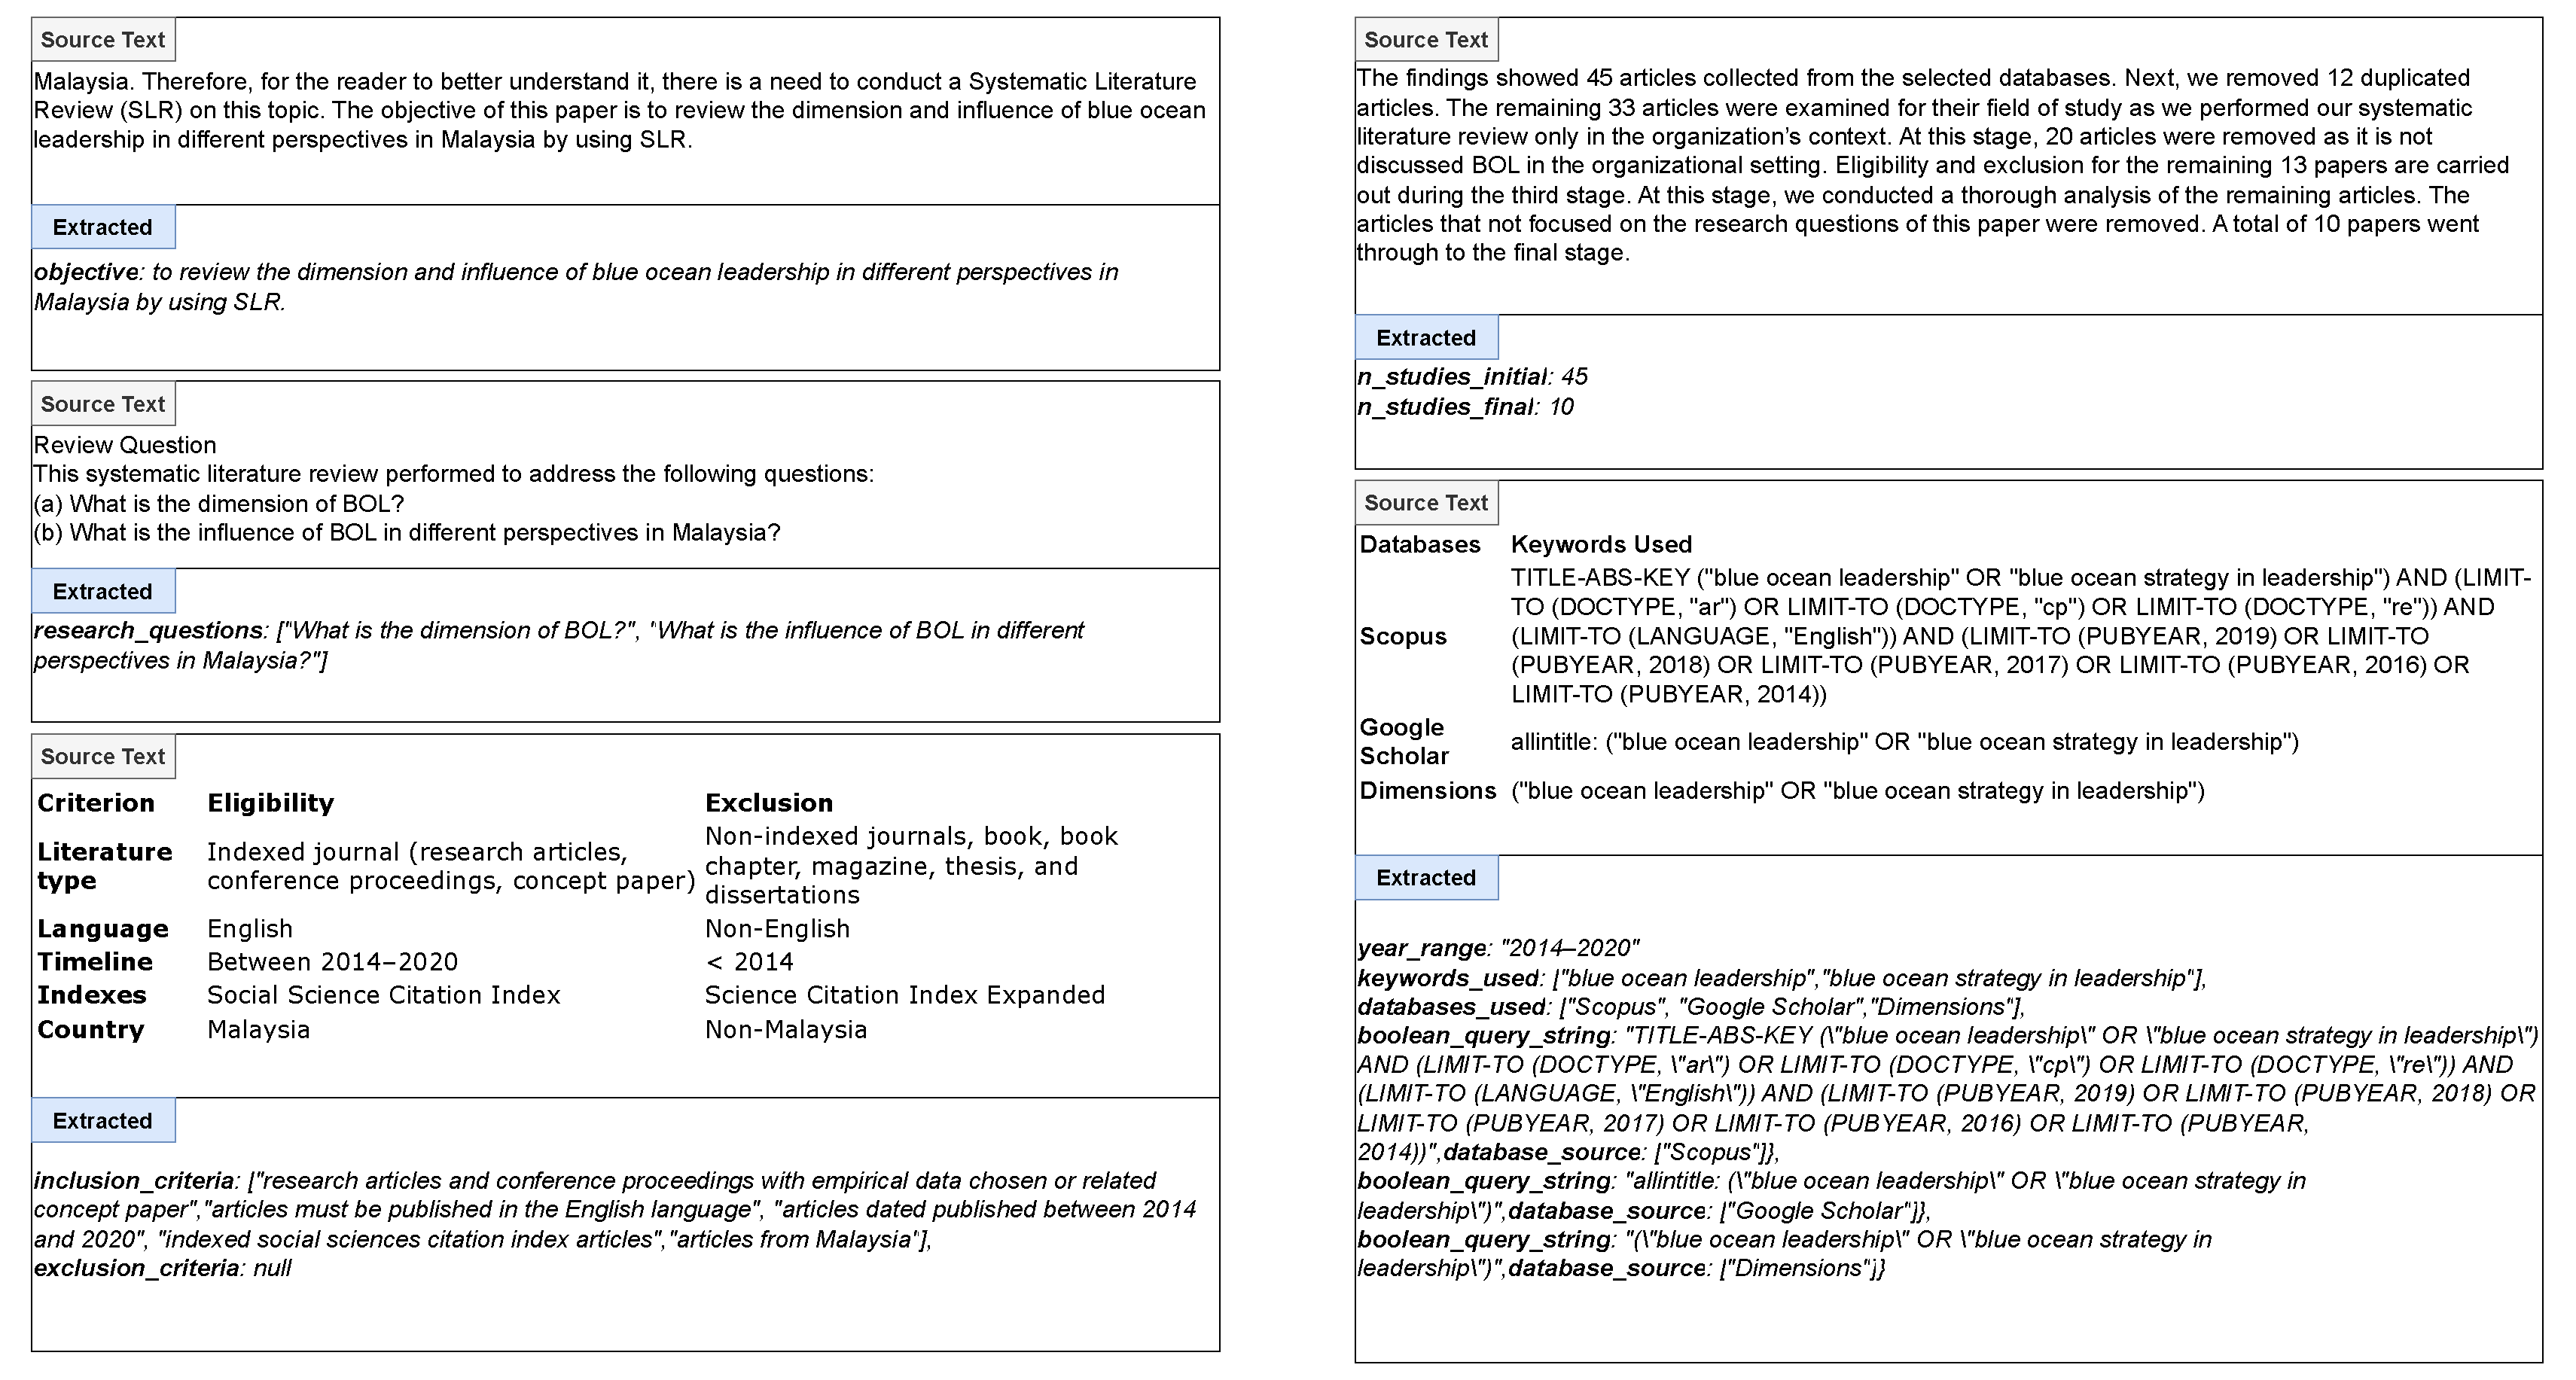
\includegraphics[width=\linewidth]{figures/example_2.pdf}
    \caption{Grounded extraction of review key information. Verbatim source spans from the PDF are transformed into structured schema fields via the verify-then-repair pipeline.}
    \label{fig:extraction_example}
\end{figure}

The final output is an evidence-centric structured representation integrating only verified extractions with OpenAlex metadata. For comparability, temporal search constraints are normalized to a canonical year-range format anchored to the publication year, while preserving original values. Table~\ref{tab:sysrev_field_coverage} summarizes metadata and methodological field coverage across the corpus after enrichment.

\begin{table}[t]
\centering
\sffamily
\renewcommand{\arraystretch}{1}
\caption{Availability of fields across \webisSRCorpus. Percentages use all 334,893 records as the denominator, except for the effectively usable subset, whose percentage uses the 107,611 records with extraction.}

\begin{tabular*}{\columnwidth}{@{\extracolsep{\fill}}lrr}
\toprule
\textbf{Subset} & \textbf{Count} & \textbf{Percentage} \\
\midrule
Total available sysrevs & 334,893 & 100\% \\
\midrule
\multicolumn{3}{l}{\textit{Availability of core materials}} \\
w/ title & 334,893 & 100.0\% \\
w/ abstract & 232,628 & 69.5\% \\
w/ extracted fields & 107,611 & 32.1\% \\
w/ all fields filled & 1,635 & 1.5\% of extracted \\
\midrule
\multicolumn{3}{l}{\textit{Review methodology fields}} \\
w/ objective & 100,203 & 29.9\% \\
w/ research questions & 17,686 & 5.3\% \\
w/ keywords used & 79,141 & 23.6\% \\
w/ boolean queries & 18,586 & 5.5\% \\
w/ inclusion criteria & 96,527 & 28.8\% \\
w/ exclusion criteria & 79,529 & 23.7\% \\
w/ date range & 334,891 & 100.0\% \\
\midrule
\multicolumn{3}{l}{\textit{Search, study-flow, and citation data}} \\
% PREVIOUSLY: \multicolumn{3}{l}{\textit{Search and study flow data}} \\
w/ databases & 98,980 & 29.6\% \\
w/ initial study count & 85,852 & 25.6\% \\
w/ final included-study count & 92,733 & 27.7\% \\
w/ resolved OpenAlex references & 334,893 & 100.0\% \\
% PREVIOUSLY:
% w/ paper counts retrieved & 85,852 & 25.6\% \\
% w/ paper counts included & 92,733 & 27.7\% \\
% w/ paper references included & 334,893 & 100.0\% \\
\midrule
\textbf{All essentials complete} & \textbf{78,058} & \textbf{72.5\% of extracted} \\
\bottomrule
\end{tabular*}
\label{tab:sysrev_field_coverage}
\end{table}


\subsection*{Query normalization}
\label{sec:query-norm}
Reported search strategies are expressed in heterogeneous, database-specific query languages, which prevents their direct execution in a single retrieval environment. To make them comparable and executable, each reported strategy is transformed into a simplified Boolean expression that can be issued to the OpenAlex API. The resulting normalized queries are included in the corpus as a separate field.

The normalization retains only topical terms and the fundamental logical operators \texttt{AND}, \texttt{OR}, and \texttt{NOT}. Database-specific syntax is removed, including explicit field tags (e.g.\ \texttt{TITLE-ABS-KEY} in Scopus or \texttt{[mesh]} in PubMed) and metadata constraints such as language or publication-type filters. Temporal restrictions are not embedded in the Boolean string; instead, the extracted year-range metadata is retained separately and can be applied externally at query time.

Normalization is performed using an instruction-tuned large language model (Qwen3-32B) applied to the reported Boolean queries or keyword lists. The model is prompted with a few-shot approach to preserve the topical vocabulary and high-level logical structure of each strategy without introducing concepts or search terms not present in the original formulation. Lightweight rule-based post-processing then ensures syntactic validity of the resulting Boolean expressions.

Some strategies cannot be normalized without additional assumptions. When numeric placeholders reference external term lists not provided in the review, or when the reported strategy contains insufficient information to construct a meaningful query, the normalized query is set to \texttt{null}. Likewise, when post-processing cannot produce a valid, non-empty Boolean expression, the query is set to \texttt{null}. Two query variants are produced where the source permits: normalized Boolean strategies reconstructed from reported search strings, and keyword-based queries constructed from reported keyword lists where a full Boolean query is unavailable.